%%%%%%%%%%%%%%%%%%%%%%%%%%%%%%%%%%%%%%%%%%%%%%%%%%%%%%%%%%%%%%%
%
% Welcome to Overleaf --- just edit your LaTeX on the left,
% and we'll compile it for you on the right. If you open the
% 'Share' menu, you can invite other users to edit at the same
% time. See www.overleaf.com/learn for more info. Enjoy!
%
%%%%%%%%%%%%%%%%%%%%%%%%%%%%%%%%%%%%%%%%%%%%%%%%%%%%%%%%%%%%%%%
\documentclass[12pt]{book}
\usepackage{graphicx}
\graphicspath{{images/}}
\usepackage{amsmath} % For the equation* environment
\usepackage{parskip}

\title{My First LaTex Document}
\author{Michael Xu\thanks{Funded by the Overleaf Team.}}
\date{June 2024}

\begin{document}
\maketitle
\tableofcontents

\part{First Part}

\chapter{First Chapter}

\section{First Section}

This is a simple paragraph at the beginning of the document. A brief introduction about the main subject.

After our abstract we can begin the first paragraph, then press ``enter'' twice to start the second one.

This line will start a second paragraph.

I will start the third paragraph and then add \\ a manual line break which causes this text to start on a new line but remains part of the same paragraph. 

Alternatively, I can use the \verb~\newline~\newline command to start a new line, which is also part of the same paragraph.

\subsection{First Subsection}

We have now added a title, author and date to our first \LaTeX{} document!
% This line here is a comment. It will not be typeset in the document.
Some of the \textbf{greatest} discoveries in \underline{science} 
were made by \textbf{\textit{accident}}.
Some of the greatest \emph{discoveries} in science 
were made by accident.
\textit{Some of the greatest \emph{discoveries} 
in science were made by accident.}

\textbf{Some of the greatest \emph{discoveries} 
in science were made by accident.}

\begin{figure}[ht]
    \centering
    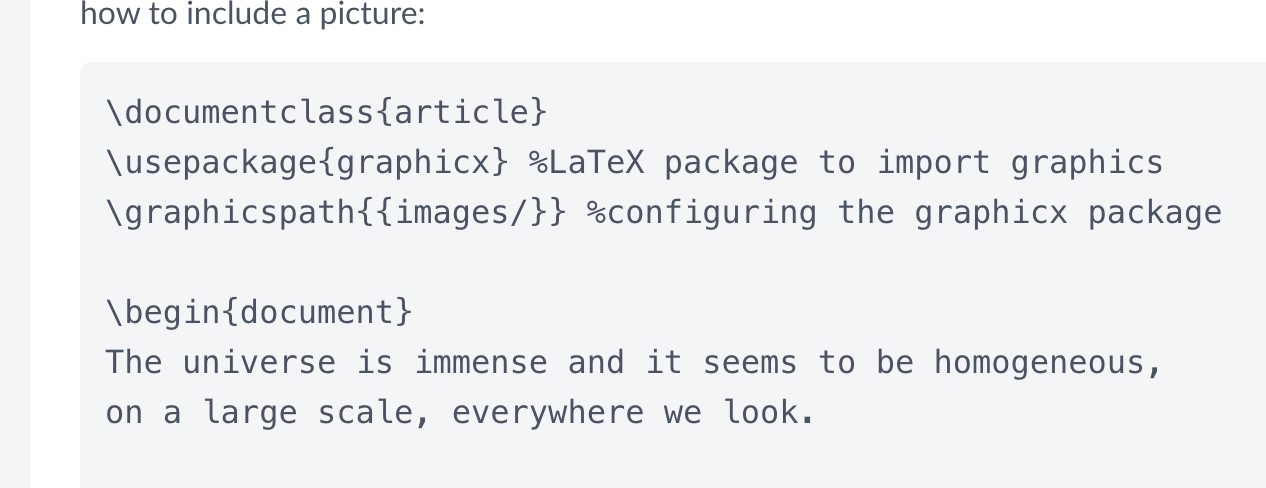
\includegraphics[width=0.80\linewidth]{screenshot}
    \caption{A nice shot.}
    \label{fig:universe}
\end{figure}

There's a picture of a galaxy above.

As you can see in figure \ref{fig:universe}, the function grows near the origin. This example is on page \pageref{fig:universe}.

\begin{itemize}
    \item he individual entries are indicated with a black dot, a so-called bullet.
    \item The text in the entries may be of any length.
\end{itemize}

\begin{enumerate}
    \item he individual entries are indicated with a black dot, a so-called bullet.
    \item The text in the entries may be of any length.
\end{enumerate}

\subsection{Second Subsection}

\begin{enumerate}
    \item he individual entries are indicated with a black dot, a so-called bullet.
    \item The text in the entries may be of any length.
\end{enumerate}

In physics, the mass-energy equivalence is stated by the equation $E=mc^2$, discovered in 1905 by \(E=mc^2\) Albert Einstein.
\begin{math}
    E=mc^2
\end{math}

\section{Second Section}

The mass-energy equivalence is described by the famous equation
\[ E=mc^2 \] discovered in 1905 by Albert Einstein. 

In natural units ($c = 1$), the formula expresses the identity
\begin{equation}
    E=m
\end{equation}

\begin{equation}
    E=m
\end{equation}

Subscripts in math mode are written as $a_b$ and superscripts are written as $a^b$. These can be combined and nested to write expressions such as

\[ T^{i_1 i_2 \dots i_p}_{j_1 j_2 \dots j_q} = T(x^{i_1},\dots,x^{i_p},e_{j_1},\dots,e_{j_q}) \]

We write integrals using $\int$ and fractions using $\frac{a}{b}$. Limits are placed on integrals using superscripts and subscripts:

\[ \int_0^1 \frac{dx}{e^x} =  \frac{e-1}{e} \]

Lower case Greek letters are written as $\omega$ $\delta$ etc. while upper case Greek letters are written as $\Omega$ $\Delta$.

Mathematical operators are prefixed with a backslash as $\sin(\beta)$, $\cos(\alpha)$, $\log(x)$ etc.

The well-known Pythagorean theorem \(x^2 + y^2 = z^2\) was proved to be invalid for other exponents, meaning the next equation has no integer solutions for \(n>2\):

\[ x^n + y^n = z^n \]

This is a simple math expression \(\sqrt{x^2+1}\) inside text. 
And this is also the same: 
\begin{math}
\sqrt{x^2+1}
\end{math}
but by using another command.

This is a simple math expression without numbering
\[\sqrt{x^2+1}\] 
separated from text.

\section{Third Section}

This is also the same:
\begin{displaymath}
\sqrt{x^2+1}
\end{displaymath}

\subsection{subsection}

\ldots and this:
\begin{equation*}
\sqrt{x^2+1}
\end{equation*}

Lorem ipsum dolor sit amet, consectetuer adipiscing elit. Etiam lobortis facilisissem...

\subsubsection{subsubsection}

\ldots and this:
\begin{equation}
\sqrt{x^2+1}
\end{equation}

Lorem ipsum dolor sit amet, consectetuer adipiscing elit. Etiam lobortis facilisissem...

\paragraph{paragraph}
Lorem ipsum dolor sit amet, consectetuer adipiscing elit. Nullam nec mi et neque pharetra sollicitudin.  Praesent imperdiet mi necante...

\subparagraph{subparagraph}
Praesent imperdietmi nec ante. Donec ullamcorper, felis non sodales...

\begin{table}
	\centering
    \begin{tabular}{l || c c r}
    	\hline
    	cell1 & cell2 & cell3 & cell4 \\
    	\hline
    	\hline
    	cell4 & cell5 & cell6 & cell 7\\
    	cell17 & cell8 & cell9 & cell 10\\
    	\hline
    \end{tabular}
    \caption{Introduce to table.}
    \label{tab:intro}
\end{table}

\section*{Unnumbered Section}
\addcontentsline{toc}{section}{* Unnumbered Section}
Lorem ipsum dolor sit amet, consectetuer adipiscing elit.  
Etiam lobortis facilisissem...

\begin{table}
    \centering
    \begin{tabular}{ccccc}
       1  & 2 & 3 & 4 & \\
       5  & 6 & 7 & 8 & \\
       9  & 1 & 2 & 3 & \\
       4  & 5 & 6 & 7 & \\
       8  & 9 & 1 & 2 & \\
       3  & 4 & 5 & 6 & \\
    \end{tabular}
    \caption{Table to test captions and labels.}
    \label{tab:data}
\end{table}

Table \ref{tab:data} shows how to add a table caption and reference a table.


\end{document}